\section{Kvadratiska ytor}
Detta är de flesta kvadratiska ytorna man kan träffa på i $\R^3$, komplett med snygga illustrationer.

\paragraph{Ellipsioider}
En ellipsioid beskrivs av en ekvation på formen
\begin{align*}
	\frac{x^2}{a^2} + \frac{y^2}{b^2} + \frac{z^2}{c^2} = 1.
\end{align*}

\begin{figure}[!ht]
	\centering
	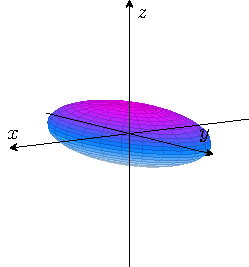
\includegraphics[scale=1]{./Images/quadric_surfaces/ellipsioid/ellipsioid.pdf}
	\caption{Illustration av en ellipsioid.}
	\label{fig:ellipsioid}
\end{figure}

\paragraph{Koner}
En kon beskrivs av en ekvation på formen
\begin{align*}
	\frac{x^2}{a^2} + \frac{y^2}{b^2} = \frac{z^2}{c^2}.
\end{align*}
\begin{figure}[!ht]
	\centering
	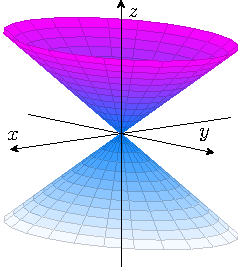
\includegraphics[scale=1]{./Images/quadric_surfaces/cone/cone.pdf}
	\caption{Illustration av en kon.}
	\label{fig:cone}
\end{figure}

\paragraph{Cylindrar}
En cylinder beskrivs av en ekvation på formen
\begin{align*}
	\frac{x^2}{a^2} + \frac{y^2}{b^2} = 1.
\end{align*}

\begin{figure}[!ht]
	\centering
	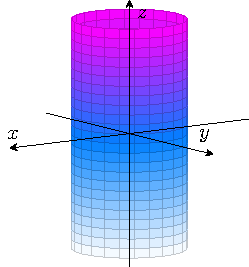
\includegraphics[scale=1]{./Images/quadric_surfaces/cylinder/cylinder.pdf}
	\caption{Illustration av en cylinder.}
	\label{fig:cylinder}
\end{figure}

\paragraph{Elliptiska paraboloider}
En elliptisk paraboloid beskrivs av en ekvation på formen
\begin{align*}
	\frac{x^2}{a^2} + \frac{y^2}{b^2} = \frac{z}{c}.
\end{align*}

\begin{figure}[!ht]
	\centering
	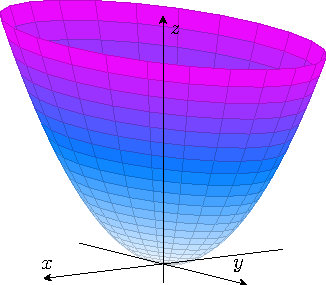
\includegraphics[scale=1]{./Images/quadric_surfaces/elliptic_paraboloid/elliptic_paraboloid.pdf}
	\caption{Illustration av en elliptisk paraboloid.}
	\label{fig:elliptic_paraboloid}
\end{figure}

\paragraph{Hyperbolska paraboloider}
En hyperbolsk paraboloid beskrivs av en ekvation på formen
\begin{align*}
	\frac{x^2}{a^2} - \frac{y^2}{b^2} = \frac{z}{c}.
\end{align*}

\begin{figure}[!ht]
	\centering
	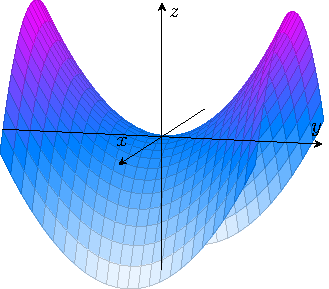
\includegraphics[scale=1]{./Images/quadric_surfaces/hyperbolic_paraboloid/hyperbolic_paraboloid.pdf}
	\caption{Illustration av en hyperbolsk paraboloid.}
	\label{fig:hyperbolic_paraboloid}
\end{figure}

\paragraph{Enmantlade hyperboloider}
En enmantlad hyperboloid beskrivs av en ekvationpå formen
\begin{align*}
	\frac{x^2}{a^2} + \frac{y^2}{b^2} - \frac{z^2}{c^2} = 1.
\end{align*}
\begin{figure}[!ht]
	\centering
	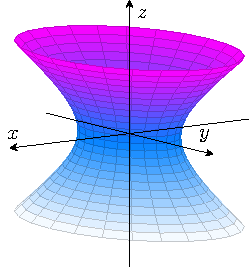
\includegraphics[scale=1]{./Images/quadric_surfaces/one_sheet_hyperboloid/one_sheet_hyperboloid.pdf}
	\caption{Illustration av en enmantlad hyperboloid.}
	\label{fig:one_sheet_hyperboloid}
\end{figure}

\paragraph{Tvåmantlade hyperboloider}
En tvåmantlad hyperboloid beskrivs av en ekvation på formen
\begin{align*}
	-\frac{x^2}{a^2} - \frac{y^2}{b^2} + \frac{z^2}{c^2} = 1.
\end{align*}

\begin{figure}[!ht]
	\centering
	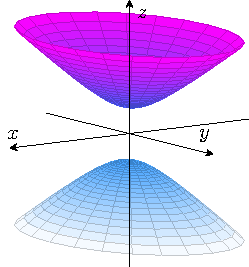
\includegraphics[scale=1]{./Images/quadric_surfaces/two_sheet_hyperboloid/two_sheet_hyperboloid.pdf}
	\caption{Illustration av en tvåmantlad hyperboloid.}
	\label{fig:two_sheet_hyperboloid}
\end{figure}